
O trabalho foi iniciado com o projeto do motor a gás frio. A seguir, este motor foi validado experimentalmente em uma bancada de teste de empuxo. Com o sistema propulsivo pronto, projetou-se o sistema de \textit{jet vanes}. Por fim, este sistema foi aferido em uma balança de três componentes para medição do empuxo e força lateral gerada pelo sistema. 

\section{Projeto do motor}\label{sec:motor_project}

O projeto do motor foi feito de maneira programática e iterativa, assegurando fácil reprodução dos resultados obtidos e automação do fluxo de dados. A linguagem de programação Julia~\cite{Julia-2017} foi utilizada para o projeto. Nesta seção, serão apresentados os dados referentes à última versão do motor. Para um histórico do desenvolvimento do motor, consultar o apêndice AAAAAAAAAAA\@.  

A tabela~\ref{tab:requirements} mostra os requisitos propulsivos, codificados PRP-N, e geométricos, codificados GMT-N, levantados para o motor. Os requisitos PRP-1 e PRP-2 foram propostos com base nos sistemas de fornecimento de ar disponíveis e na escala desejada do motor. Já a temperatura do propelente, requisito PRP-2, é baseada na temperatura ambiente, e permite a utilização de \textit{jet vanes} feitas de materiais simples. Com base nestes requisitos, um sistema monopropelente a ar foi proposto. Os requisitos GMT-1 e GMT-2 foram especificados com base na necessidade de haver estagnação na câmara de empuxo (seção~\ref{sec:intro}) e na necessidade de fácil manipulação, manufatura e conexão. Já os requisitos GMT-3 e GMT-4 buscam propiciar um escoamento com alto paralelismo na região da tubeira, assim como facilitar a manufatura.

\begin{table}[htpb]
    \centering\begin{tabular}{cccc} \toprule
        Código & Variável & Grandeza & Valor \\ \midrule
        PRP-1 & \(P_C\) & Pressão de câmara & \(500\;\mathrm{kPa}\) \\
        PRP-2 & \(T\) & Empuxo & \(2\;\mathrm{N}\) \\
        PRP-3 &\(T_{prop}\) & Temperatura do propelente & \(298,15\;\mathrm{K}\) \\
        GMT-1 & \(r_{C,\text{min}}\) & Raio de câmara mínimo & \(15\;\mathrm{mm}\) \\
        GMT-2 & \(L_C\) & Comprimento de câmara & \(30\;\mathrm{mm}\) \\
        GMT-3 & \(\alpha_{\text{conv}}\) & Semi-ângulo do convergente & \(30\mathrm{^\circ} \) \\
        GMT-4 & \(\alpha_{\text{div}}\) & Semi-ângulo do divergente & \(5\mathrm{^\circ} \) \\ \bottomrule 
    \end{tabular}
    \caption{Requisitos propulsivos e geométricos para o motor.}\label{tab:requirements}
\end{table}

A partir destes requisitos, o software CEA NASA foi utilizado para calcular os parâmetros propulsivos (\(\varepsilon \), \(C^\ast \) e \(C_f\)) do sistema com pressão ambiente \(P_{amb} = 100kPa\). Com estes coeficientes, pode-se aplicar as relações~\ref{eq:exp_ratio} e~\ref{eq:C_F} descritas na seção~\ref{sec:intro} para calcular as áreas de saída \(A_e\), de garganta \(A_t\). A área de câmara, \(A_C\), foi calculada diretamente a partir do requisito GMT-1. Foi introduzida uma seção cilíndrica na garganta do motor, com área de seção transversal \(A_t\), para garantir a manufatura precisa dessa dimensão.

Os três coeficientes propulsivos calculados também foram utilizados para estimar o fluxo mássico de propelente \(\dot{m}\), e este, para estimar a velocidade do propelente na mangueira de alimentação, \(v_{\text{prop}}\). Estes parâmetros são relevantes para a verificação da perda de carga no sistema de alimentação, bem como para a escolha da fonte de ar. Como o propelente é pouco energético, altas vazões são necessárias mesmo para empuxos pequenos, de modo que conhecer a capacidade exigida da fonte foi fundamental. A partir de \(\dot{m}\), cujo cálculo foi descrito anteriormente, e assumindo que a  um diâmetro de tubo \(d\), massa molar do ar \(\mathrm{MM}_{ar}\) e constante dos gases \(R\):
\begin{equation}
    v_{\text{prop}} = \frac{\dot{m} R T_{\text{prop}}}{\pi {\left(\frac{d}{2}\right)}^2 P_C \mathrm{MM}_{ar}}
\end{equation}

Com as áreas das seções transversais do motor calculadas, e em posse da especificação da geometria interna do motor, gerou-se o CAD do motor para impressão 3D. Em Julia, utilizou-se a package \textit{ConstructiveGeometry}\footnote[1]{https://github.com/plut/ConstructiveGeometry.jl} para gerar a geometria tridimensional a partir do dados de geometria calculados. Ao produzir o CAD diretamente a partir do código de projeto, foi possível eliminar etapas manuais que podem introduzir erros e atrasos ao projeto. A impressão 3D foi escolhida como método de manufatura devido à baixa temperatura de operação do motor, e à sua geometria complexa, assim como pela velocidade de prototipagem propiciada por esta tecnologia. O material de impressão usado foi ABS\@. Para evitarem-se vazamentos, a impressão 3D foi feita com uma configuração de impressão de cinco perímetros, ou seja, com 5 camadas externas contínuas seguindo os contornos da geometria. Esta configuração foi escolhida iterativamente com base em resultados intermediários obtidos.

\section{Validação do projeto do motor}\label{sec:method_validation}

O motor projetado e impresso em 3D foi montado em uma bancada de testes e instrumentado com os sensores da tabela ref. Os sensores, bem como uma válvula de gás comandada eletronicamente, foram ligados a um Arduino Mega para leitura e controle do conjunto de testes. 

%https://www.arduino.cc/reference/en/libraries/max6675/

\begin{table}[htbp]
    \centering\begin{tabular}{p{0.15\textwidth}p{0.5\textwidth}p{0.2\textwidth}} \toprule
        Sensor & Montagem & Biblioteca usada \\ \midrule
        Termopar & Inserido lateralmente na câmara de empuxo, selado com cola de ABS & MAX6675 \\
        Célula de carga & Apoio para o motor, sentido de medida paralelo ao empuxo & HX711 \\
        Transdutor de pressão & Acoplado à câmara de empuxo em furo lateral; ver CAD na seção RESULTADOS & Leitura analógica simples \\ \bottomrule
    \end{tabular}
    \caption{Descrição dos periféricos usados nos testes de validação do motor desenvolvido.}\label{tab:validation_peripherals}
\end{table}

Para o controle da bancada foi desenvolvida uma \textit{command line interface} simples para permitir testes interativos. Assim, as funções de tara, calibração, abertura e fechamento de válvula e leitura de sensores podiam ser comandadas a partir de uma interface textual interativa que facilitou a iteração do teste.

\section{Projeto do sistema de \textit{jet vanes}}\label{sec:method_jet_vanes}

Devido à disponibilidade de materiais, foi utilizada uma lâmina de aço de 0,7mm de espessura como \textit{jet vane}. Com este sistema, desejou-se a capacidade de posicionar a lâmina defletora com resolução de \(1^\circ \), com alcance de deflexão de \(\pm 20^\circ \). Também foi necessário projetar um suporte para o motor que permitisse a conexão da mangueira de alimentação de gás. Por fim, este sistema deveria ter um encaixe circular de \(12mm\) para um eixo de acoplamento com a balança de três componentes, conforme descrito na seção~\ref{sec:method_3axis_measurement}. Durante o projeto do sistema, levou-se em consideração a factibilidade de manufatura, bem como a necessidade de acesso ao servomotor e ao motor foguete para desmontagens e trocas.

Para o projeto mecânico do sistema, foi usado o sistema CATIA\@. Para a deflexão da lâmina defletora, escolheu-se um servomotor de aeromodelismo devido à acessibilidade deste componente bem como à sua resolução angular, que satisfaz o requisito exposto acima. As peças foram todas impressas em 3D com ABS\@.

\section{Caracterização do sistema em balança de três componentes}\label{sec:method_3axis_measurement}

Um sistema de vetorização de empuxo planar, como o desenvolvido neste trabalho, produz de modo geral uma força longitudinal, paralela ao empuxo do motor foguete, uma força transversal, gerada pela lâmina defletora, e um torque, causado pelas forças aerodinâmicas atuantes sobre a lâmina defletora, bem como pelo desalinhamento da força total gerada em relação a um ponto de medida. Sendo assim, é necessário que sejam medidas três grandezas para a caracterização do sistema, ou seja, uma força longitudinal, uma força transversal e um torque. Empiricamente, é possível também medir três forças e, através do cálculo de forças totais e binários, extrair as forças e momentos do sistema. Este tipo de medição é bastante comum em aerodinâmica, onde perfis de asas devem ser caracterizados quanto ao seu arrasto, sustentação e momento~\cite{anderson}.

Sendo assim, o sistema desenvolvido foi acoplado à balança de três componentes disponível no Laboratório Feng, exibida na figura~\ref{fig:3axis_scale}. Apesar de montada a um túnel de vento, este não foi utilizado no experimento.

\begin{figure}[htbp]
    \centering
    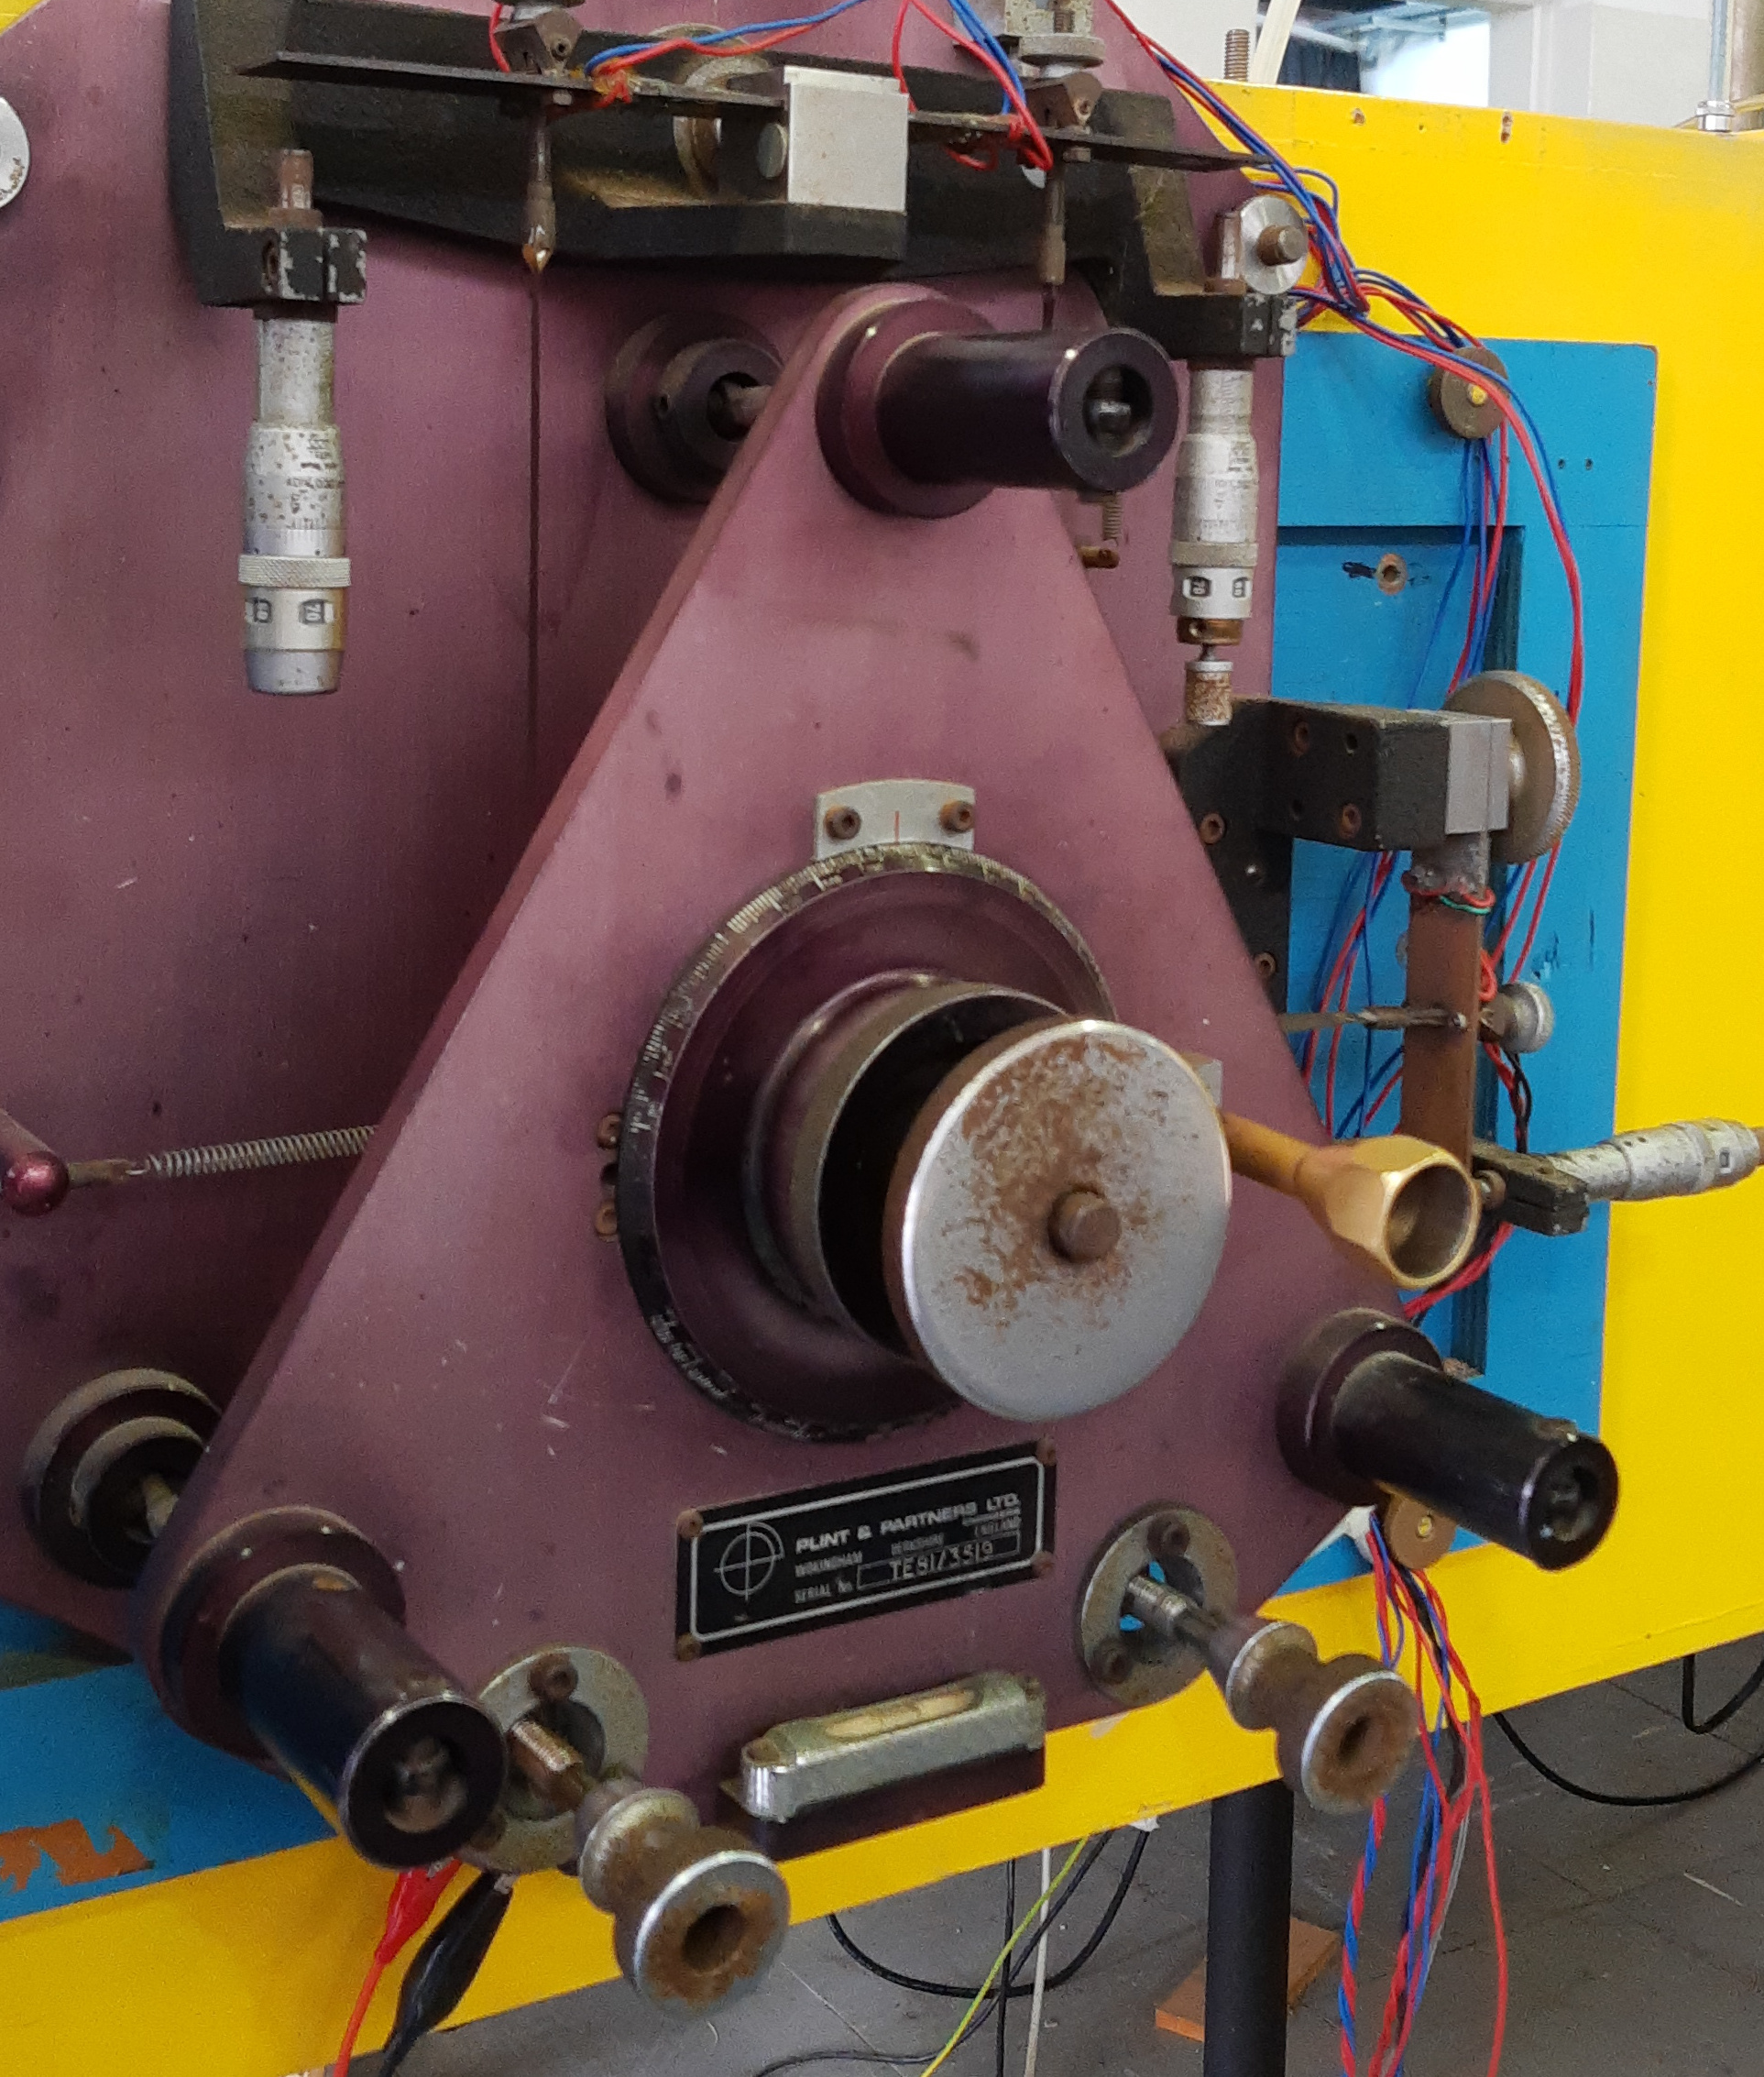
\includegraphics[width=\textwidth]{img/eixocropped.jpg}
    \caption{Balança aerodinâmica utilizada para o experimento.}\label{fig:3axis_scale}
\end{figure}

A balança apresenta uma zona morta, o que significa que para baixos carregamentos a leitura é quase nula. Por isso, e também devido às baixas forças envolvidas no experimento, a balança foi pré-carregada com pesos externos para garantir linearidade, com a configuração dos pesos mostrada na figura~\ref{fig:pre_loading}. Os pesos nos pratos azul (canto inferior esquerdo) e prata (ao lado da balança, entre os trilhos pretos verticais) foram escolhidos como metade do fundo de escala da balança. A calibração foi feita modificando os pesos aplicados nestes pratos, conforme discutido adiante.

\begin{figure}[htbp]
    \centering
    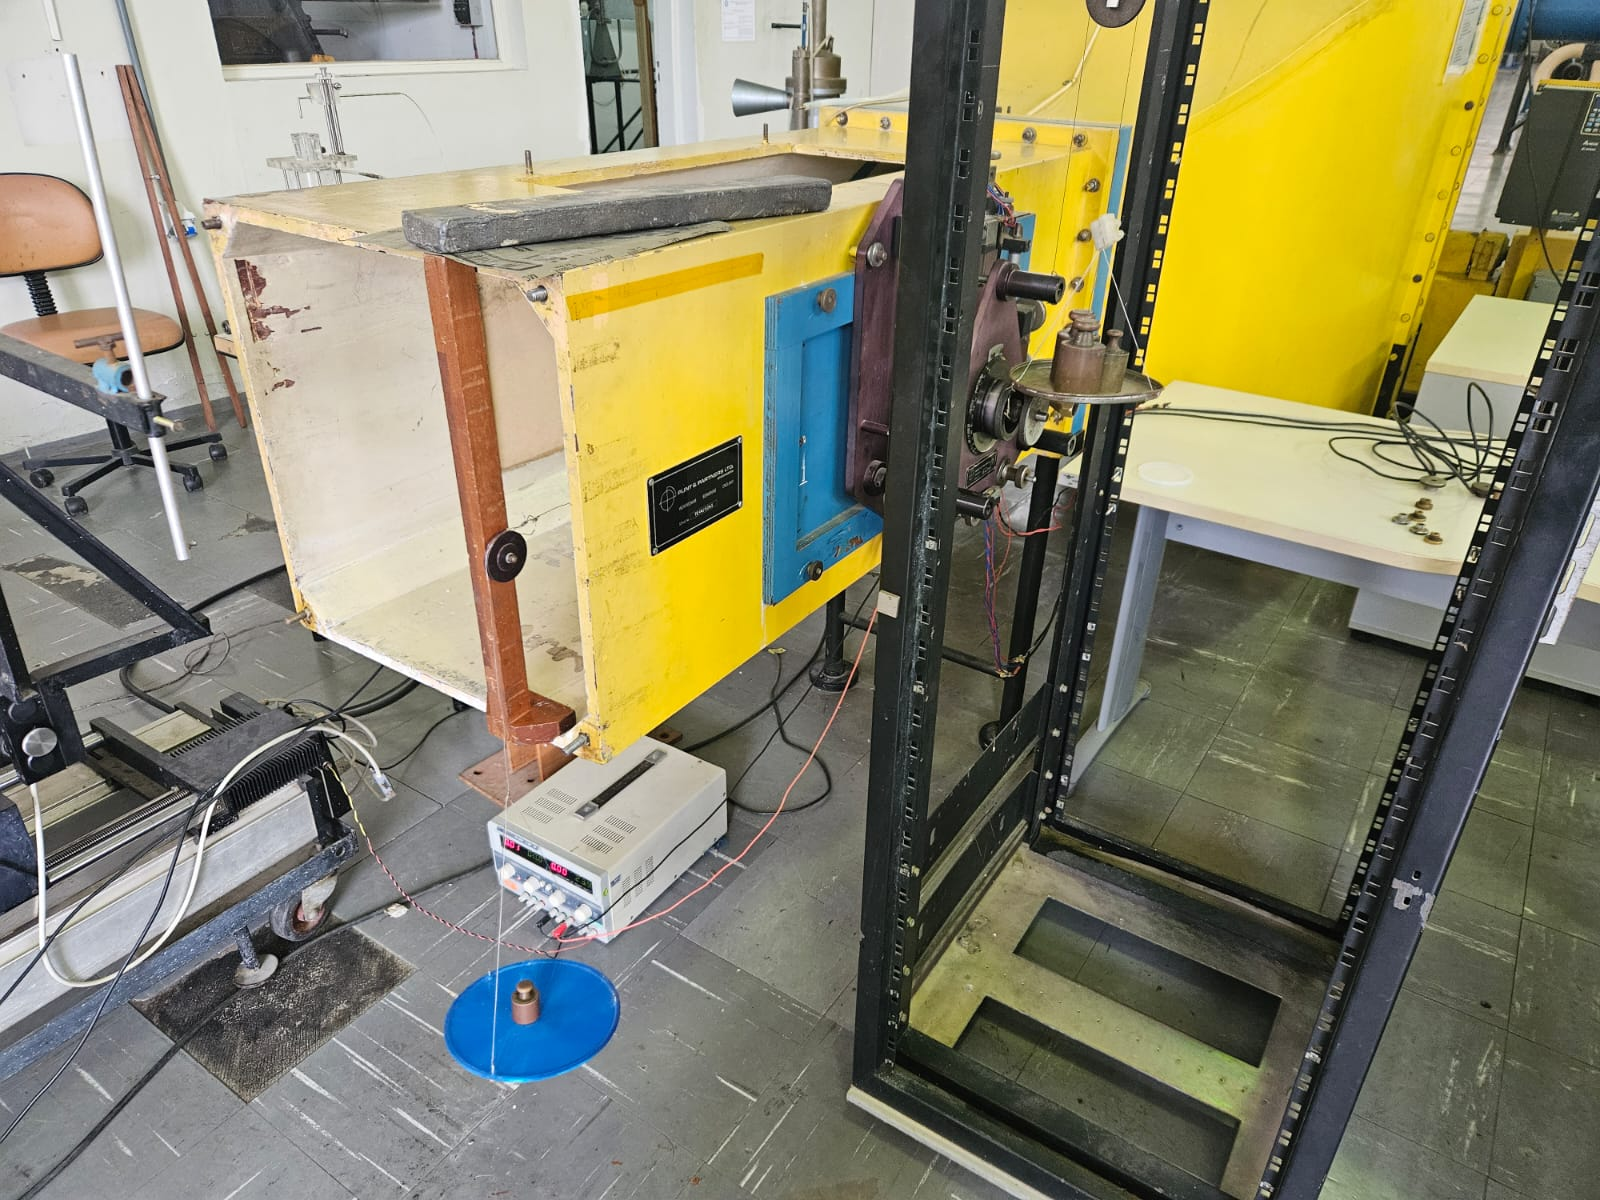
\includegraphics[width=\textwidth]{img/montagem_externa.jpeg}
    \caption{Configuração do pré-carregamento da balança de três componentes.}\label{fig:pre_loading}
\end{figure}

Dentro da seção de teste, o sistema de vetorização de empuxo foi montado como na figura~\ref{fig:montagem_interna}. Para uma explicação mais detalhada do sistema, ver seção~\ref{sec:result_jet_vanes}. O motor foi posicionado na vertical, com seu eixo de maior força coincidindo com o eixo de maior fundo de escala da balança. A tubeira do motor foi apontada para uma direção sem impedimentos para o fluxo, de modo a minimizar vibrações e interferências mecânicas no experimento. Na figura, é possível observar também os fios de controle do servomotor (cabeamento branco, preto e vermelho), bem como a mangueira de alimentação de gás do motor (parte inferior da imagem). O eixo que pode ser visto na figura~\ref{fig:montagem_interna} está encaixado no furo central da balança, facilmente visível na figura~\ref{fig:3axis_scale}.

\begin{figure}[htbp]
    \centering
    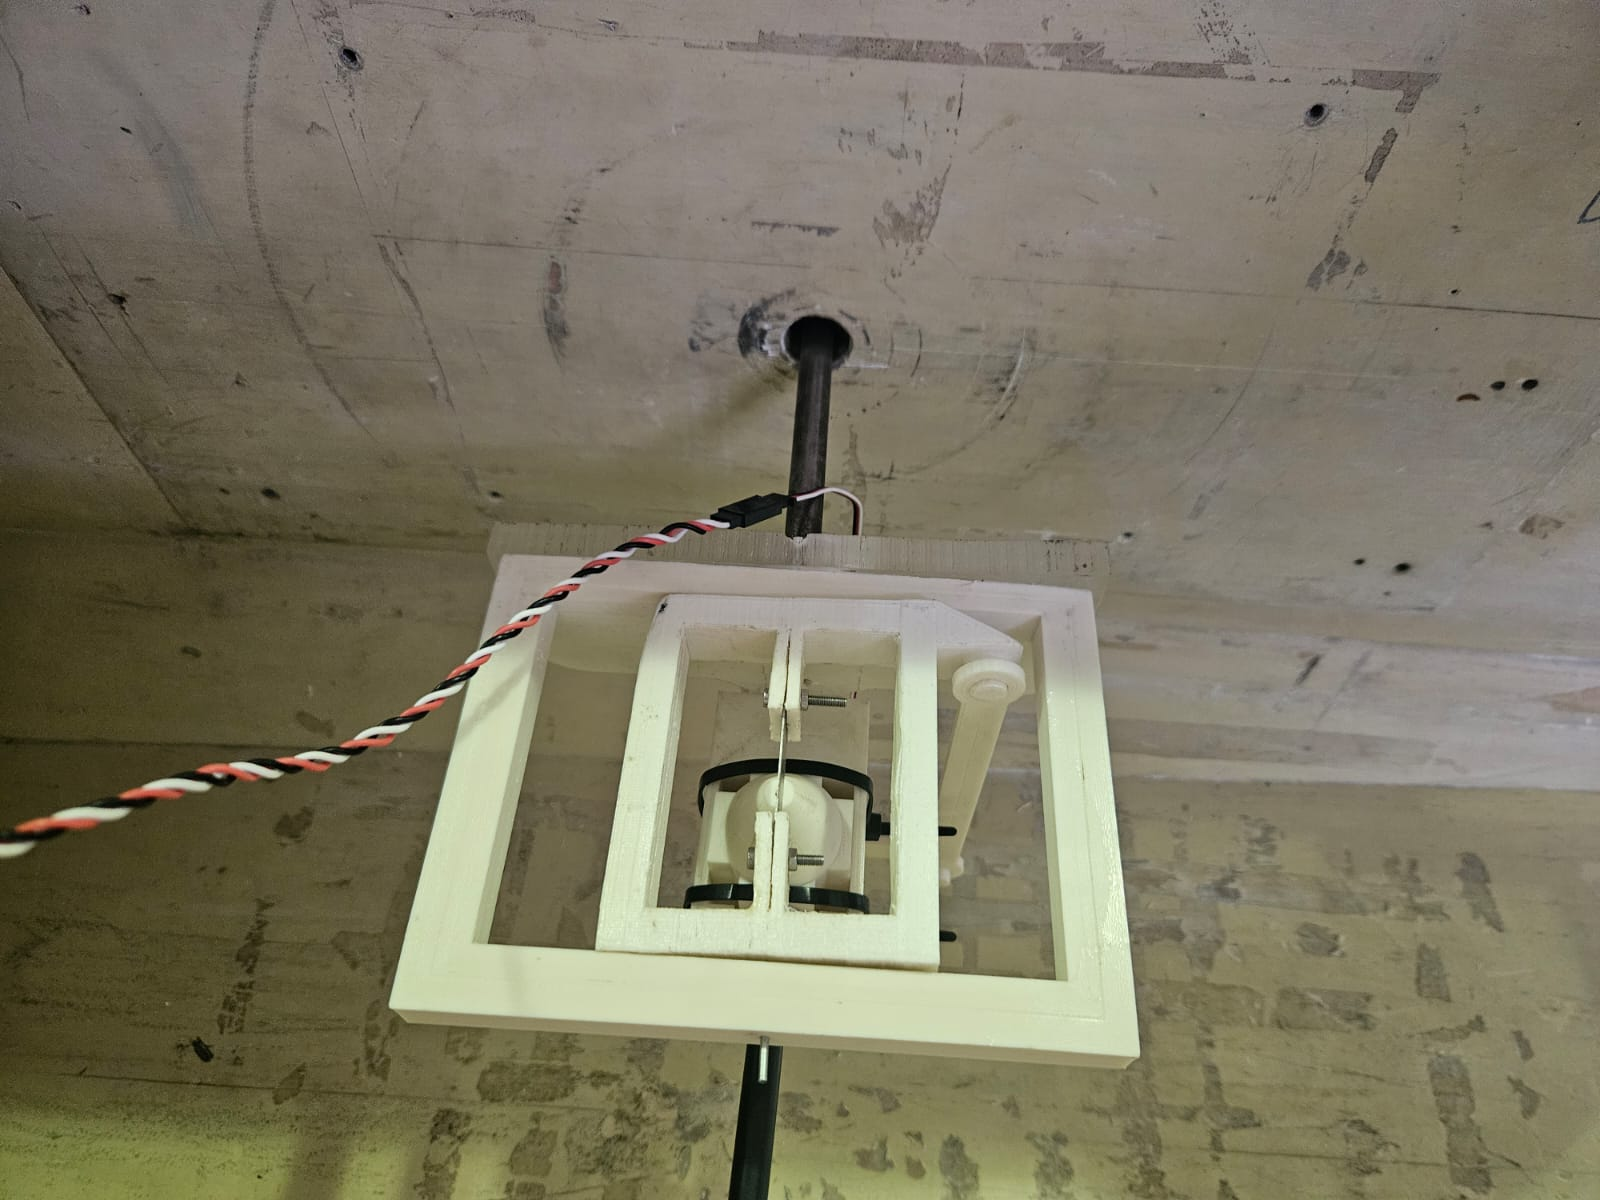
\includegraphics[width=\textwidth]{img/montagem_interna.jpeg}
    \caption{Montagem do sistema de vetorização de empuxo na balança de três componentes}\label{fig:montagem_interna}
\end{figure}

A balança possui três células de carga, conforme visto na figura~\ref{fig:scale_diagram}. Destas células de carga são obtidas as forças \(F_x\), \(F_y\) e o torque \(M\) gerado sobre o eixo através das relações~\cite{lab}:
\begin{align}
    F_A &= F_y + \frac{2M}{d} \label{eq:FA}\\
    F_F &= F_y - \frac{2M}{d} \label{eq:FF}\\
    F_D &= F_x \label{eq:FD}
\end{align}
onde \(F_A\), \(F_F\) e \(F_D\) representam respectivamente as forças aplicadas sobre as células \textit{aft} (traseira), \textit{fore} (frontal) e \textit{drag} (de arrasto) e \(d\) é a distância entre as células de carga A e F. 

\begin{figure}[htbp]
    \centering
    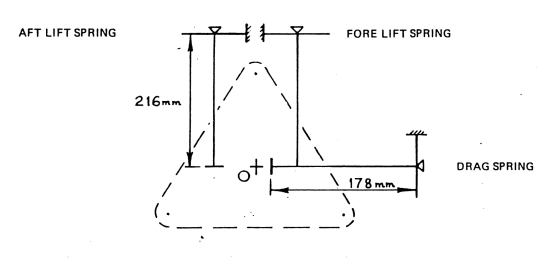
\includegraphics[width=\textwidth]{img/three_axis_scale_diagram.png}
    \caption{Diagrama esquemático da balança de três componentes.}
    \label{fig:scale_diagram}
\end{figure}

Para a calibração da balança, deve-se relacionar as forças sobre as células de carga com as tensões lidas pelo sistema de aquisição de dados. Para este experimento, a existência da mangueira de alimentação de gás apresentou um problema empírico devido à sua rigidez e forma natural. Portanto, a balança foi calibrada com pesos conhecidos (aplicando-se forças \(F_x\) e \(F_y\), que carregam as três células de carga) com o sistema conectado à mangueira, para evitar grandes fontes de erros sistemáticos. Observa-se que a pressurização da mangueira introduz mais rigidez e desloca o equilíbrio da balança, de modo que ainda existem erros sistemáticos na calibração feita. As forças foram aplicadas modificando os pesos colocados nos pratos da figura~\ref{fig:pre_loading}. Para cada peso aplicado, foram coletadas as leituras dos três componentes e, com as forças calculadas para cada componente através das equações~\ref{eq:FA} a~\ref{eq:FD}, foi feito um ajuste linear por mínimos quadrados entre a saída da balança (tensão) e a carga aplicada.

Após a calibração da balança, foi medida a força gerada pelo motor foguete sem lâmina defletora para estabelecer uma medida de controle sobre o alinhamento do motor e a vazão mássica oferecida pelo sistema de ar comprimido usado. Em seguida, a lâmina defletora foi montada novamente e foram extraídas curvas de forças e torque em função de sua deflexão, controlada pelo servomotor. Pensando na possibilidade de haver alguma folga mecânica que prejudicasse o prosicionamento preciso da lâmina, foram extraídas curvas através da varredura de ângulos em sentido crescente e decrescente. Ou seja, se com o servomotor em \(90\mathrm{^\circ}\) a lâmina está paralela ao escoamento que sai da tubeira, foram feitas varreduras de \(70\mathrm{^\circ}\) a \(110\mathrm{^\circ}\), bem como de \(110\mathrm{^\circ}\) a \(70\mathrm{^\circ}\).